\title{Star Formation and Feedback in Stellar Clusters and Galaxies}

\author{PI: Mordecai-Mark Mac Low, American Museum of Natural History, New York.\\
        co-PIs: Andrew Emerick, Columbia University / AMNH, Joshua Wall, Drexel University / AMNH}

\documentclass[11pt]{article}

\usepackage[letterpaper, margin=1in]{geometry}
\usepackage{amsmath}

\usepackage{natbib}
\usepackage{multirow}
\usepackage{multicol}
\usepackage{array}
\usepackage{graphicx}
\usepackage{epstopdf}
%\usepackage{siunitx}
\epstopdfsetup{update}
\newcolumntype{L}{>{\centering\arraybackslash}m{2cm}}
\newcolumntype{R}{>{\centering\arraybackslash}m{1.25cm}}

\renewcommand{\floatpagefraction}{.8}%

\citestyle{aa}

\newcommand {\apj}{ApJ}
\newcommand {\aj}{AJ}
\newcommand {\apjs}{ApJS}
\newcommand {\apjl}{ApJL}
\newcommand {\mnras}{MNRAS}
\newcommand {\aap}{A\&A}
\newcommand {\aapr}{A\&ARv}
\newcommand {\araa}{ARA\&A}
\newcommand {\pasj}{PASJ}
\newcommand {\pasp}{PASP}
\newcommand {\bain}{Bulletin of the Astronomical Institutes of the Netherlands}
\newcommand {\fcp}{Fundamentals of Cosmic Physics}
\newcommand {\nat}{Nature}
\newcommand {\na}{New Astronomy}
\newcommand{\eg}{e.g.,}
\newcommand\rmxaa{Rev. Mex. Astron. Astrofis.} % Revista Mexicana de Astronomia y Astrofisica

%\DeclareSIUnit\parsec{pc}
\newcommand{\msun}{$\textrm{M}_{\odot}$}
\newcommand{\rsun}{$\textrm{R}_{\odot}$}
\newcommand{\lsun}{$\textrm{L}_{\odot}$}

\begin{document}
\maketitle

\section{Introduction}
%{\bf actual draft of this section pending Josh's end:}
This renewal proposal describes our proposed research for the coming year in two related areas of astrophysical research. The PI of this proposal (M-M. Mac Low) is PI on NSF grant AST11-09395, which also supports co-PI Wall, while co-PI Emerick is supported by a NSF Graduate Research Fellowship (DGE-16-44869).
Our research focuses on understanding the precise effects of feedback physics 
using detailed models in two distinct regimes: cluster formation in giant molecular clouds (lead by co-PI Wall), and
star formation histories of low mass dwarf galaxies (lead by co-PI Emerick). 
% AE: made parenthetical consistency 

Both projects represent novel endeavors in their respective sub-fields. The cluster formation simulations combine stellar dynamics and evolution with a detailed feedback model in a hybrid hydrodynamics/N-body simulation reaching down to resolutions of hundreds of AU.  Our dwarf galaxy simulations also include feedback at a coarser scale of 1.5~pc in a model tracking individual stars---unique on galactic scales---while also tracking stellar yields to trace both gas and stellar phase abundances for a dozen distinct metal species. Each project is supervised by PI M-M. Mac Low, with collaborator S. McMillan co-advising the cluster project, and collaborator G. Bryan co-advising the dwarf galaxy project. We summarize the science motivation for each of these projects below, while justifying our resource request. We note that each of these projects is central to the PhD thesis of each of the co-PIs.
% AE: changed "one" to "each" in the above.... I am assuming this is for Josh's thesis work as well?
% Wall (GMC's) and co-PI Emerick (dwarf galaxies).

\subsection{Star Cluster Formation in Giant Molecular Clouds}

Star cluster formation theory is at an exciting threshold. Over the last decade, theorists studying the interstellar medium (ISM) have conducted increasingly sophisticated simulations of molecular cloud formation and evolution, increasing both the dynamic range of simulations and the number of physical effects modeled. Simulations of molecular clouds now include supernovae, flux frozen magnetic fields, and detailed chemistry all in a single simulation \citep{Klessen_2000_GasDynTurb,MacLow2004,Joung2006,Hill2012,Ibanez-Mejia2016,haid_supernova-blast_2016,Walch_SILLC1}. Simultaneously, the size and physical complexity of star cluster simulations has also increased, with the first million body simulation of a star cluster recently performed \citep{Dragon_Wang}, which included stellar evolution, binary formation and mass transfer, and GPU accelerated integration of stellar motion. 

The intersection of these two fields comes when newly formed stars interact with the surrounding gas through the effects of winds, radiation, and supernovae, collectively described as stellar feedback, while the inhomogeneous gas exerts tidal forces on the newly forming cluster. Numerical algorithms modeling stellar feedback have seen a great deal of recent attention. Supernova methods have become increasingly better at reproducing observations at all times, with recent kinetic energy injection models capturing the temperature and density evolution from pre-Sedov phase to cold remnant \citep{Simpson2015,Kim_Ostriker_2015ApJ}. Winds have been modeled often in stellar feedback simulations as either pure thermal energy injection or actual kinetic particle injection \citep{Pelupessy_embedded_SC,Dale_winds_2013}. Finally radiation has been modeled with numerous different algorithms such as ray tracing and the M1 closure and including either thermal heating, radiation momentum pressure, or both \citep{Dale_Winds_and_H2,WiseAbel2011,RAMSES-RT,Raskutti_Ostriker_2016}.

However simulating star cluster formation is a complex problem. While many of the above simulations contain the specific physics of one or two forms of feedback, all three forms are expected to be present during the first 10--15~Myr %\SIrange{10}{15}{Myr} 
of a new cluster's existence \citep{Krumholz2014}. Complex N-body dynamics also occur, forming and dissolving binaries that can lead to mass transfer and altered stellar evolution in the system \citep{PortegiesZwart2007}. Finally, many of the simulations of star cluster formation cited above start from idealized initial conditions. This usually consists of a spherical density distribution with a turbulent velocity spectrum \citep{Dale_Winds_and_H2,Raskutti_Ostriker_2016}, instead of gravitationally-formed filamentary structures \citep{Ibanez-Mejia2016} that are subjected to ongoing external stellar feedback from supernovae \citep{Hill2012} and other mechanisms. For simulations that do start with more realistic initial gas distributions, stars are generally not individually resolved but are represented in groups of stars by cluster particles \citep{Gatto_Walch_SILCC3_2016,dobbs_properties_2016}.

\subsection{Star Formation, Feedback, and Chemodynamics of Galaxies}

Recently, large scale, cosmological hydrodynamics simulations have been able to reproduce many observed, integral properties of galaxies over a wide range of galaxy stellar masses and dark matter halo masses \citep[\eg][]{MUGS2010, MAGICC2013, Illustris1, Illustris2, OWLS, EAGLE, FIRE, APOSTLE, Latte}. 
%mm [redundant with following sentence]  These works have made strides in reconciling outstanding disagreements between predictions from $\Lambda$CDM cosmology and observations of nearby dwarf galaxies. 
Improvements in our understanding of baryonic physics, most importantly understanding the importance of stellar feedback in self-regulation of star formation in galaxies, has allowed these works to reconcile many outstanding disagreements between predictions from $\Lambda$CDM cosmology and observations of nearby dwarf galaxies. However, due to computational constraints, feedback implementations are usually phenomenological, tuned to reproduce observed galaxy properties. Clearly, given its role in galaxy evolution, a deeper understanding of feedback physics is needed. This can be gained through high resolution, idealized simulations of individual galaxies. We propose to conduct a sensitive test of how various feedback processes affect galaxy evolution in order to self-consistently reproduce dynamical, morphological, and chemical properties of dwarf galaxies simultaneously. We will conduct high resolution simulations of small dwarf galaxies, varying the underlying feedback physics, while, for the first time in a galaxy scale simulation including well-resolved feedback, tracing chemical abundances and stellar evolution on a star-by-star basis.

Historically, inclusion of feedback physics in galactic scale simulations meant the injection of purely thermal energy in a localized region---often with tricks to prevent rapid, unphysical overcooling of gas---to model the effects of supernovae explosions. It has become clear that feedback physics must be implemented in much greater detail than this, simultaneously considering multiple, distinct types of feedback energy. In addition to energy injection from core collapse and Type Ia supernovae, we will include the effects of 1) energy injection from the winds of both massive and AGB stars, 2) radiation feedback (photoionization, photoheating, and radiation pressure) from massive stars followed directly using adaptive ray tracing, 3) a model for photoelectric heating of dust grains due to stellar radiation, and 4) cosmic rays (CRs) injected at supernova sites, which provide a non-thermal additional pressure in the ISM. The effect of these feedback sources on the chemical evolution of galaxies will provide a new dimension of analysis and observational comparisons not often considered in these types of simulations.

In general we have a fair understanding of the mean chemical properties of galaxies, but models have difficulty in reproducing the observed scatter in both gas phase and stellar abundances. In particular, models of the chemical evolution of dwarf galaxies are often tuned to match the observed properties of a small number of observed galaxies. Self-consistently reproducing both the dynamic and chemical, or chemodynamical, properties of dwarf galaxies in hydrodynamics simulations remains a standing challenge for theoretical models. In addition, with one exception \citep{Few2012, Few2014}, all hydrodynamics simulations examining galactic chemodynamics to date have been implemented in smooth particle hydrodynamics (SPH) codes. Although historical problems with the SPH formalism have been ameliorated substantially in recent years, they often still employ sub-grid mixing schemes to model mixing of spatially adjacent but chemically inhomogeneous gas \citep[\eg][]{ShenWadsleyStinson2010}. In part due to these methods, there are outstanding uncertainties in how much results depend on specific code implementations \citep{Revaz2016}. In addition, using star particles that represent clusters of stars becomes problematic at the high spatial and particle mass resolution needed for simulating low mass dwarf galaxies \citep{Revaz2016}. 

This motivates our development and use of a new method for studying galactic chemical evolution in hydrodynamics simulations, including, for the first time, a broad range of feedback physics, while also following individual stars down to the solar mass range. This is particularly exciting with recent or ongoing---for example ANGST \citep{ANGST2009}, APOGEE \citep{APOGEE2010}, and GAIA---and upcoming observational studies (e.g. APOGEE-2) that will obtain stellar abundance measurements in both the Galaxy and nearby dwarfs. These will provide ideal comparisons to our simulations of dwarf galaxies with individual, chemically tagged stars.

We provide a discussion of the feedback physics and associated models we propose to include in our simulations. We seek to understand how each of these processes individually and together affect galactic dynamical and chemical structure. 

\section{Technical Goals}

\subsection{Towards More Realistic Star Cluster Formation}

To conduct more realistic star cluster simulations we have integrated the (R)MHD code Flash into the Astrophysical Multipurpose Software Environment(AMUSE) \citep{AMUSE}, an astrophysics software package that contains community codes for hydrodynamics, N-body dynamics, stellar evolution and radiative transport. This allows us to include accurate N-body dynamics for the stars using the GPU accelerated code ph4 \citep{ph4}. We have also augmented the publicly available version of Flash itself to include modules for radiation (momentum and heating), winds and supernova. Radiation is tracked using an improved version of the FERVENT module \citep{baczynski_fervent:_2015}. For supernova we have implemented the kinetic energy injection method of \citet{Simpson2015}, and for winds we use our own adaptation of the \cite{Simpson2015} method, injecting winds as a mixture of both kinetic and thermal energy. We will use this more realistic model of stellar feedback to study the impact of newly formed stars on their environment by analyzing how stellar formation efficiency evolves near natal clusters, how turbulence is driven by feedback, and whether any ejected or impacted gas can lead to or disrupt further star formation. 

\subsection{Galactic Feedback Physics}

The following physics will be identical in each galactic simulation: 1) gas self-gravity to capture gas collapse and subsequent star formation in dense regions, 2) a nine-species, non-equilibrium chemistry solver, following electrons, and H, He, and H$_{2}$ and their ionization states \citep{Anninos1997, Abel1997}, 3) associated heating / cooling as followed in the \texttt{Grackle} library (Smith et al.\ in prep), including heating from a metagalactic UV background \citep{HM2012} and tabulated metal line cooling from \texttt{Cloudy} \citep{Cloudy2013}, 4) approximate H and He gas self-shielding of the UV background \citep{Rahmati2013}, 5) a metagalactic Lyman-Werner (LW) flux from \cite{HM2012} to properly model H$_{2}$ dissociation, as well as an optically thin LW flux from each of our stars to account for local fluctuations in the LW field, and 6) a collisionless N-body solver to evolve the dynamics of the formed star particles. In every simulation, we form stars from dense gas on the most refined parts of the grid (with resolution of 1.5~pc) following a stochastic star formation scheme from \cite{Goldbaum2015, Goldbaum2016}, modified to sample individual stellar masses from an input IMF \citep[e.g.][]{Salpeter1955}. Each star is chemically tagged by the local gas abundances, and assigned stellar properties from a grid of stellar evolution tracks \citep{Bressan2012}, which ultimately govern the radiative properties of the stars (if radiation feedback is used), the stellar wind velocity, and the star's lifetime. We follow the mass loss of each particle via stellar winds and supernovae over time as determined by our stellar yield model.

Since they are the sources of chemical enrichment in galaxies -- our key observational discriminator between feedback mechanisms -- supernovae and stellar wind feedback will be treated uniformly in all simulations. Stellar yields for both winds and supernovae are taken from the NuGrid data set \citep[][, Ritter et. al. in prep]{Pignatari2016}, a self-consistent model of stellar yields over a well sampled range of stellar masses ($M_{*} \in [1,25]~M_{\odot}$) and metallicities ($Z\in [10^{-4},0.2]$). We model stellar winds from massive stars ($M > 8~M_{\odot}$) using a constant mass loss rate over their lifetime, while low mass stars ($M < 8~M_{\odot}$) remain quiescent until a final AGB phase wind emitted near the end of their lives. Stellar properties, including lifetimes,  start of a star's AGB phase, radius, surface gravity, and effective temperature are obtained via interpolation over the \texttt{PARSEC} grid of stellar evolution tracks \citep{Bressan2012}\footnote{Stellar radius, surface, gravity, and effective temperature are used only for determining radiation properties of our stars, and play no direct role in our simulations}. Stars below 8 M$_{\odot}$ are tracked after their death as white dwarf particles, assigning white dwarf masses from the observed initial-to-final-mass distribution \citep{Salaris2009}. Following \citep{Cote2015}, we use an observationally motivated delay time distribution model \citep[\eg][]{Maoz2014} to assign to each white dwarf a time when they will explode as a Type Ia supernova.\footnote{We note that only a few percent of white dwarfs should explode as Type Ia in a Hubble time \citep{Maoz2014}; our model takes this into account in assigning explosion times, with a large majority never exploding.} We adopt Type Ia supernova yields from \cite{Thielemann1986}.

Accounting for the effects of CRs in galaxy scale simulations has only been possible recently, yet is likely a very important source of additional feedback in galaxies \citep[\eg][]{SalemBryan2014, SalemBryanHummels, SalemBryanCorlies, GirichidisCR, Pakmor2016, Simpson2016}. The role of CRs in low mass dwarf galaxies is still uncertain, though has been investigated recently in more massive dwarfs than those considered in this proposal \citep{Chen2016}. The implementation of CR feedback in \texttt{Enzo} \citep{SalemBryan2014} assumes both isotropic diffusion and ignores energy losses from interactions with an ordered magnetic field. Isotropic diffusion in very low mass dwarf galaxies may not be a poor assumption, as their lack of obvious disk structure may indicate that they lack the ability to create a global, ordered magnetic field that would cause anisotropies in CR behavior. We inject CR energy during supernova explosions at 10\% of the total energy injected, reducing the subsequent thermal / kinetic energy injection accordingly. CRs in our simulations diffuse isotropically as controlled by a diffusion coefficient, and interacting with the hydrodynamics through an additional, non-thermal pressure term.

Radiation from massive stars provides a substantial additional source of feedback in galaxies \citep[\eg][]{Agertz2013}. Including radiative feedback has a significant affect on galaxy dynamical and morphological structure \citep[\eg][]{WiseAbel2012, Kim2013a, Kim2013b, Roskar2014, Rosdahl2015}. Radiation fluxes for each of our stars are computed using the \texttt{OSTAR2002} grid of stellar atmosphere models \citep{Lanz2003}; for stars with effective temperatures below those sampled on the \texttt{OSTAR2002} grid, we compute radiation rates assuming a black body spectrum, scaled to be consistent with the \texttt{OSTAR2002} models. In this proposal, we include radiative feedback in two distinct forms: 1) H and He ionizing radiation from massive stars, and 2) local FUV flux from all stars that contributes to photoelectric heating within the ISM. Separating these physics will allow us to directly address recent disagreement in the role of photoelectric heating in dwarf galaxies \citep{Hu2016, Forbes2016}. We use \texttt{Enzo}'s radiative transfer capabilities \citep{Wise2012a,WiseAbel2012,Wise2014} to track ionizing radiation directly, coupling the ionizing / heating rates to the \texttt{Grackle} chemistry solver, and accounting directly for the effects of Hydrogen radiation pressure. We assume the FUV radiation to be everywhere optically thin and apply a photoelectric heating rate model from \cite{BakesTielens1994} and \cite{Wolfire2003} that scales with local density, temperature, and metallicity.

%\section{Computational Methods}

%\subsection{Flash}

%Flash is a magnetohydrodynamics (MHD) code with adaptive grid refinement \citep{FLASH}. Magnetohydrodynamics is an approximation to solving the full charged, multi-species fluid problem. The problem is assumed to be electrically neutral on any scale large enough to be relevant to the simulation. But there can be flows of charged particles in different directions (known as the one fluid model) which act like a current and result in magnetic fields. These fields in turn effect the fluid and evolve in time according to the MHD equations. FLASH solves the conservative MHD equations given as (shown here in dimensionless form with extensive variables being per unit mass)


%\begin{widetext}
%\begin{eqnarray}
%\frac{\partial \rho}{\partial t} + \nabla \cdot \left(\rho \vec{v} \right) &=& 0 \\
%\frac{\partial \rho \vec{v}}{\partial t} + \nabla \cdot \left(\rho \vec{v} \vec{v} - \vec{B} \vec{B} \right) + \nabla p_{tot} &=& \rho \vec{g} + \nabla \cdot \tau \\
%\frac{\partial \rho E}{\partial t} + \nabla \cdot \left[\vec{v} \left(\rho E + p_{tot} \right) - \vec{B} \left(\vec{v} \cdot \vec{B}\right)\right] &=& \rho \vec{g} \cdot \vec{v} + \nabla \cdot \left(\vec{v} \cdot \tau + \sigma \nabla T \right) + \nabla \cdot \left[ \vec{B} \times \left( \eta \nabla \times \vec{B} \right) \right] \\
%\frac{\partial \vec{B}}{\partial t} + \nabla \cdot \left(\vec{v} \vec{B} - \vec{B} \vec{v}\right) &=& - \nabla \times \left(\eta \nabla \times \vec{B}\right) 
%\end{eqnarray}
%\end{widetext}

%\noindent
%where

%\begin{eqnarray}
%p_{tot} &=& p + \frac{B^2}{2} \\
%E &=& \frac{1}{2}v^2 + \epsilon + \frac{B^2}{2 \rho} \\
%\tau &=& \mu\left[\nabla \vec{v} + \left(\nabla \vec{v}\right)^T - \frac{2}{3}\left(\nabla \cdot \vec{v}\right) \mathbf{I} \right]
%\end{eqnarray}

%\noindent
%gives the total pressure (thermal plus magnetic), the total energy, and the viscous stress respectively and $\mathbf{I}$ is the identity matrix, $\epsilon$ is the specific internal energy and $\vec{g}$ is the body force per unit mass due to gravity (or other forces if present). Note that in determining magnetic fields in GMCs usually the plasma $\beta$ is given

%\begin{equation}
%\beta = \frac{2p}{B^2}
%\end{equation}

%\noindent
%which is the ratio of the thermal pressure to the magnetic pressure. For GMCs this value is $\sim$ 0.04 \citep{Crutcher_1999}. We can then use this value to estimate the initial magnetic field in a GMC from the pressure.

%The simulation domain is represented in Cartesian coordinates as a grid of blocks, where each block is constructed of a cube of cells. Refinement occurs at the block level when a refinement criterion is met, such as the gradient in density of the fluid across two cells becoming too large. If the criterion are satisfied, the refined block is divided into eight blocks, (for a 3 dimensional grid) since the block is split in two in each dimension. Refinements are nested, with the newly created child blocks connected to the parent blocks in a tree structure for interpolation and prolongation across refinement levels.

%\subsection{ph4}

%For the N-body dynamics we have chosen the GPU accelerated parallel code ph4 \citep{ph4}, which combines the direct summation of the gravitational acceleration with a 4th order Hermite integration. This method predicts the acceleration and jerk analytically, then applies a corrector to the acceleration and jerk with Hermite interpolation of the second and third derivatives of the acceleration \citep{Makino4thHermite}. This method is more accurate than the basic leap frog integrator contained in FLASH, which will allow us to resolve close encounters.


%When two (or more) bodies do have a close encounter in PH4, the encounter will be handed off the Multiples module in AMUSE \citep{AMUSE}, which solves the few body problem for the interaction as a separate process. Once the encounter resolves, both objects will then integrated back into PH4 either as a single object if a binary formed, or two separate objects with the proper trajectories if they did not. Finally, stellar and binary evolution in the simulation will be obtained from the code SeBa \citep{Portegies_SeBa}. This will give the location of each star on the main sequence, allowing us to then input radiation and winds into FLASH for each star accurately, as well as detect when a supernova event occurs and simulate this in FLASH appropriately.

\subsection{Gravity Bridge}

To couple Flash (RMHD) to ph4 (N-body), we have implemented a momentum and energy conserving gravity bridge \citep{Fujii_Makino_bridge} which is a symplectic second order method first used to integrate the solar system \citep{Wisdom_Holman_1991}. This allows the two codes to evolve independently for multiple hydrodynamic and dozens or hundreds of N-body timesteps (which we call a ``drift"), after which the mass in each code gives a gravitational acceleration to the other (a ``kick"). Both codes evolve independently in parallel during the drift, with the N-body portion (ph4) running on GPUs, and Flash on CPUs.

% AE: This paragraph isn't entirely clear.. I'd reword, but I'm not entirely sure what it should say
We have tested the conservation of both energy and momentum in this method. Figure \ref{fig:ener} shows energy conservation to follow the behavior of the 4th order Hermite method \citep{binney2011galactic}, with global error on the order of 0.5\%. The momentum error is dominated by other factors in the code such as accretion onto sink particles, and is globally on the order of 1\% (Fig \ref{fig:mommod}).

\begin{figure}
\centering
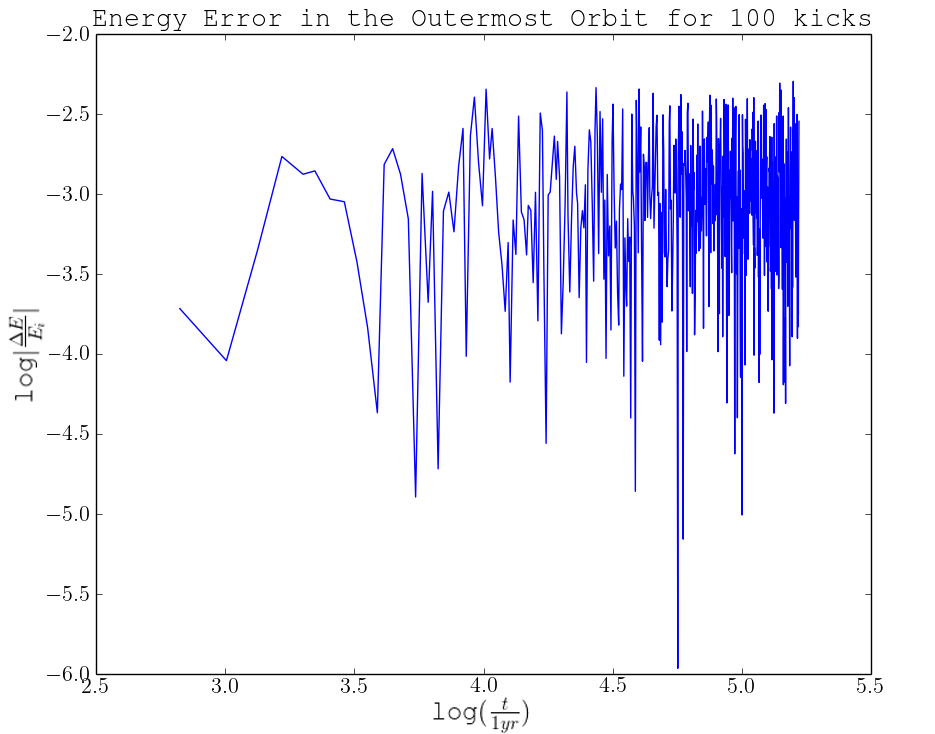
\includegraphics[width=0.75\linewidth]{ener_mod}
\caption{\small Energy error of the Flash/ph4 gravity bridge via AMUSE for the orbit of three sink particles through a stationary isothermal gas sphere. The bridge timestep was step such that the outer particle recieved 100 kicks per orbit.}
\label{fig:ener}
\end{figure}

\begin{figure}
\hspace{-1.0cm}
\centering
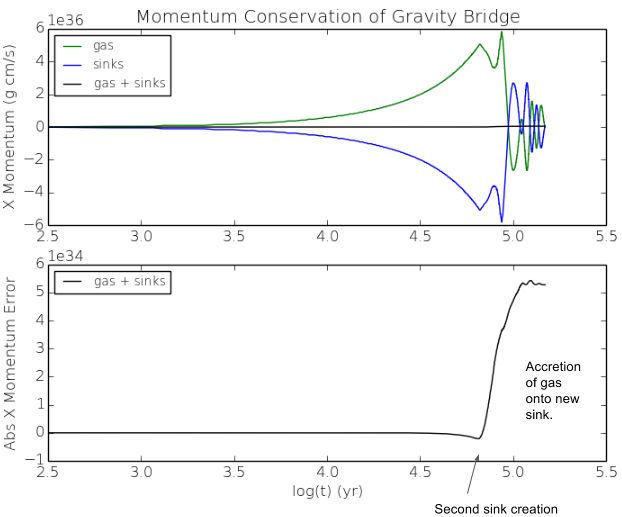
\includegraphics[width=0.75\linewidth]{mom_mod}
\caption{\small The total momentum and momentum error for a simulation starting with a spherical gas clound and a sink using the Flash/ph4 gravity bridge via AMUSE. The gas cloud collapses and forms a second sink during the run. Note the y axis scaling, the error is two orders of magnitude smaller than the total momentum. The primary error comes from accretion onto the newly formed sink particle and is a ``worst case scenario" for our code.}
\label{fig:mommod}
\end{figure}

\section{Model Descriptions}
\subsection{Stellar Clusters}

% AE: could be a little stronger, but I'm not familiar with the work to edit safely
We will be zooming in on high fidelity ISM simulations run by Juan Iba\~{n}ez-Mej\'{i}a \citep{Ibanez-Mejia2016}. These MHD simulations start with a 1x1x40 kpc elongated box representing a slice of a spiral galaxy gas disk. Initially the gas is stirred by supernova injected energy for approximately 200~Myr without gravity. Then both self gravity and a Navarro-Frenk-White (NFW) dark matter background are switched on and molecular clouds and cloud complexes form. These clouds have densities and velocity dispersions consistent with observations, with many undergoing collapse which would lead to star formation. Several molecular clouds from these simulations would be appropriate for our study, ranging in mass from %\SIrange{1e3}{1e6}{\msun}.
$10^3$--$10^6$~\msun.  We have developed code which zooms in on selected clouds gradually, allowing for the turbulent energy to naturally cascade down to our final resolution. We intend to zoom in on three of these clouds: one $8 \times 10^3$~{\msun} cloud, one $10^5$~{\msun} cloud, and one cloud complex that is $10^6$~{\msun}. %The first cloud is shown in Fig \ref{fig:bullhead}.

%\begin{figure}
%\centering
%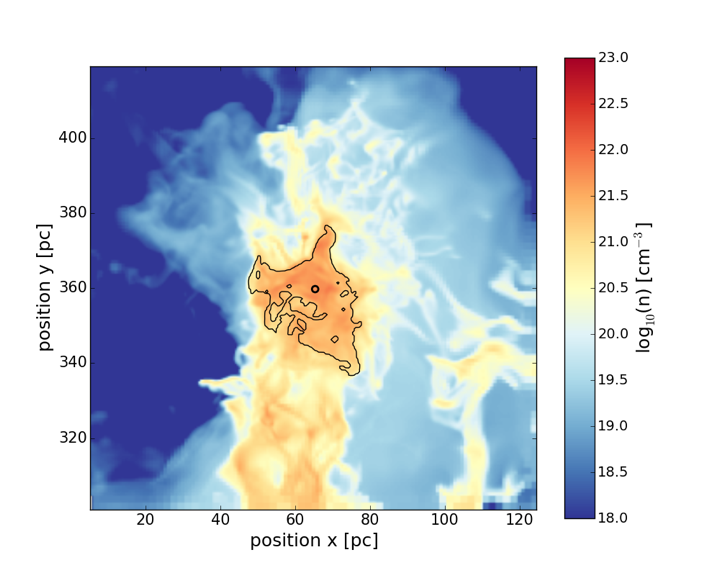
\includegraphics[width=0.7\linewidth]{bullhead_mod}
%\caption{\small Integrated column density of the ``Bullhead" cloud, which is $8 \times 10^3$~{\msun}. The contour shown is at $n~=~10^3~{\rm cm}^{-3}$.}
%\label{fig:bullhead}
%\end{figure}

\subsection{Dwarf Galaxies}
Our dwarf galaxy simulations will be carried out using \texttt{Enzo}\footnote{www.enzo-project.org}, an adaptive mesh refinement (AMR) hydrodynamics and N-body code. \texttt{Enzo} is an entirely open-source code that is undergoing active development by many researchers across several institutions; its most recent stable release is version 2.5. This project involves a substantial amount of additional code development built on top of the development version of \texttt{Enzo} (version 2.X)\footnote{This version is also publicly available at www.bitbucket.org/aemerick/enzo-emerick}. \texttt{Enzo} has been well tested and extensively used in a variety of applications, including the ISM \citep{2005MNRAS.356..737S, 2008ApJ...673..810T}, the IGM \citep{2000ApJ...534...57B, 2001ApJ...561L..31F}, the first stars and galaxies \citep[\eg][]{Wise2012a, WiseAbel2012, Wise2014}, and the roles of various feedback methods in galaxies \citep[\eg][]{Simpson2015, SalemBryan2014, Goldbaum2016, Forbes2016}. We outline the methods employed in \texttt{Enzo} as relevant to our proposal; a detailed description of these methods can be found in the \texttt{Enzo} method paper \citep{Enzo2014}. 

To produce a controlled set of numerical experiments on the effect of various feedback physics on galaxy evolution, we will begin by initializing our galaxy as a spheroidal gas cloud embedded in a dark matter background potential, and simulate it through collapse until just before first star formation, using a halo virial mass of $10^{9}$ M$_{\odot}$ and gas mass of $\sim10^{7}$ M$_{\odot}$. These initial conditions will be held fixed for all subsequent models. These masses are chosen to be consistent with what the Local Group ultrafaint dwarf galaxy Leo P \citep{McQuinn2013, Giovanelli2013, Skillman2013, McQuinn2015} may have had prior to star formation (the current gas mass of Leo P is about 10$^{6}$ M$_{\odot}$). The collapsed gas cloud will serve as the initial conditions from which we will vary the underlying feedback physics. Differences in the subsequent evolution will be analyzed to understand the role of each feedback mechanism. 

We center each dwarf galaxy on a uniform $128^3$ cell mesh with physical dimensions of $12.288^3$ kpc, corresponding to a root grid resolution of 96 pc. Additional levels of refinement are applied to regions surpassing a chosen density contrast, in addition to requiring the Jeans length be resolved to at least 16 cells. Each additional level of refinement increases the resolution by a factor of 2, allowing us to achieve 1.5 pc resolution with a total of 6 levels of refinement. In addition, we force refinement around all star particles, so that feedback injection is always resolved at the maximum refinement level. Ideally we would like to use higher resolution in order to completely resolve key aspects of the feedback physics (particularly relating to bubble formation from stellar winds and ionizing radiation); however this becomes exceedingly expensive to run for gigayear timescales. Such long timescales are essential to capture a long period of star formation evolution and chemical enrichment; $\sim$ 1 Gyr represents a few dynamical times in our dwarf galaxy, the time required to understand metal mixing across the galaxy. In addition, 1 Gyr is approximately the timescale over which the knee in the $\left[ \alpha / \rm{Fe}\right]$ vs. $\left[\rm{Fe}/\rm{H}\right]$ diagram appears, marking the time when substantial iron peak elemental enrichment from Type Ia supernovae begins. Capturing this knee is an important observational diagnostic.

Based on our tests at 1~and 2~pc resolution, 1.5~pc resolution both adequately resolves these feedback physics, and remains computationally tractable to run for our required timescales.. \texttt{Enzo} helps reduce overall expense by using adaptive time steps, evolving each refinement level independently with the timestep size set by the Courant-Friedrichs-Levy condition for numerical stability for that level. The exact size of each step is thus dependent on the sound speed and gas velocity in zones at that level. Since supernova can heat the ISM to temperatures on order of 10$^{6-7}$ K, and stellar winds have velocities on order of 10$^{3}$ km s$^{-1}$, we expect typical timesteps of about 600 years on our most refined level.

We couple \texttt{ENZO} to the open-source \texttt{Grackle} chemistry and heating/cooling library, which operates cell-by-cell on each grid. \texttt{Grackle} sub-cycles through a non-equillibrium chemistry solver following methods first used in \cite{Anninos1997} and \cite{Abel1997} that solve for the correct densities and ionization states of each species, while accounting for radiative cooling and heating from external radiation fields. This allows us to self-consistently couple our 9 species chemistry network with the heating/cooling effects from the metagalactic background, and galactic ionizing, far-ultraviolet, and LW radiation fields.
%mm , and  photoelectric heating from the far-ultraviolet radiation field.

CR's are traced using the two-fluid approximation implemented in \cite{SalemBryan2014}. The CRs are treated as a secondary fluid coupled to the hydrodynamics through a pressure term, acting as an additional, non-thermal pressure source. CR diffusion is computed with an explicit finite difference scheme, which places an additional constraint on the size of each timestep, though the impact of this constraint is reduced somewhat by subcycling over the CR evolution. The CR timestep scales with the square of the cell size and is inversely proportional to the adopted diffusion coefficient. For a diffusion coefficient of $3\times10^{28}$~cm$^{2}$~s$^{-1}$, this corresponds to a reduction of a factor of $\sim$5 in our typical time step size over runs without CR's. For example, we expect typical time steps of $\sim$600 yr due to stellar winds at 1.5 pc resolution; including CR's, the diffusion limited timestep at this resolution is 112.5 yr at maximum resolution. We note that this impact is greatest at the highest refinement level: the hydrodynamics timestep decreases by a factor of two with doubled resolution, while the CR diffusion substep decreases by a factor of four, showing the need for subcycling.

We use the direct ray tracing algorithm described by \cite{WiseAbel2011} in \texttt{Enzo} to directly follow the H~{\sc i} and He~{\sc i} ionizing radiation from massive stars. This is an adaptive ray tracing method that splits rays using mapping on a \texttt{HEALPix} grid. These methods are well tested and have been used previously in cosmological simulations of reionization in the early Universe \citep{Wise2012a, WiseAbel2012,Wise2014, Kim2013a, Kim2013b}. These methods have been demonstrated to scale to $\mathcal{O}(10^{3})$~processors for large domains (up to $\sim 10^9$ cells) and many sources ($\sim10^{4}$). Although we expect $\sim$100-500 sources at any one time in our simulations, direct ray tracing does still incurs a significant additional expense. We mitigate this additional expense by allowing rays to merge once they are far from their source, and using a reduced speed of light approximation (though we are capable of running without this simplification); neither of these approximations should significantly affect results in an isolated galaxy simulation. As discussed in our supplemental code scaling document, with these approximations we anticipate a slow down of a factor of 5--10 for our typical source count.

Figure~\ref{fig:dwarf galaxy} shows the results from a low resolution (8 pc) proof-of-concept simulation of our dwarf galaxy model about 60 Myr after the onset of star formation. Shown are face-on slices of number density (top left), temperature (top right), and H~{\sc i} ionizing radiation (bottom left), as well as an edge-on full box projection showing total carbon column density (bottom right). Each of the 4,324 star particles (total mass of $1.2\times10^4$ M$_{\odot}$) in this snapshot are marked with a small, black dot; 173 of these particles are radiation sources. This simulation was run on 64 processors on the TACC Stampede cluster, where we propose to work.

\begin{figure}
\centering
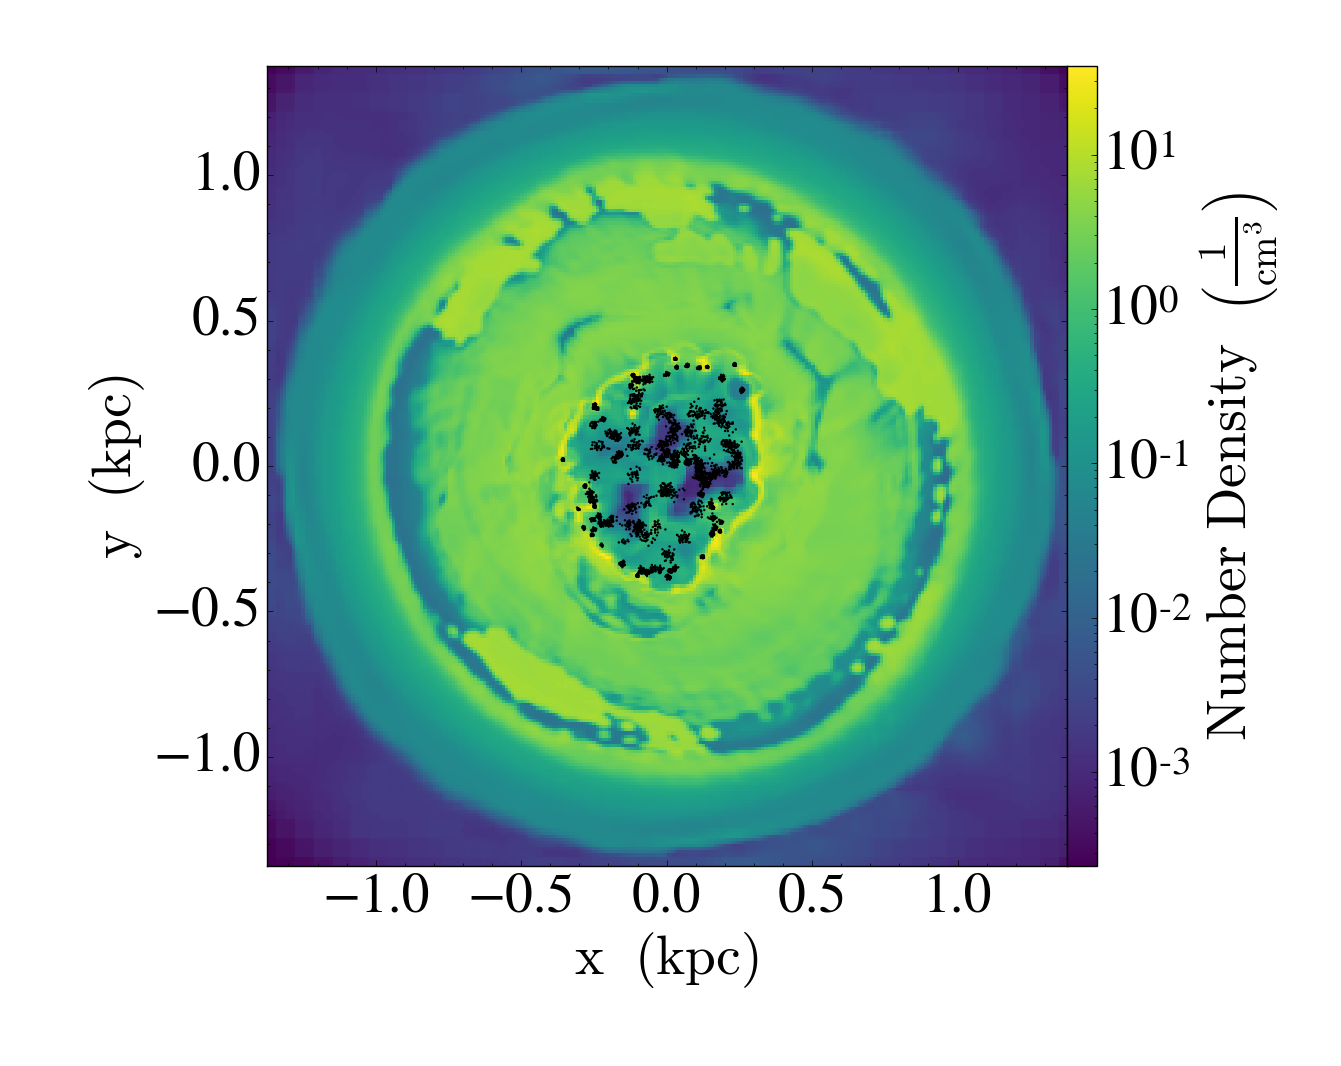
\includegraphics[width=0.4\linewidth]{number_density_slice}
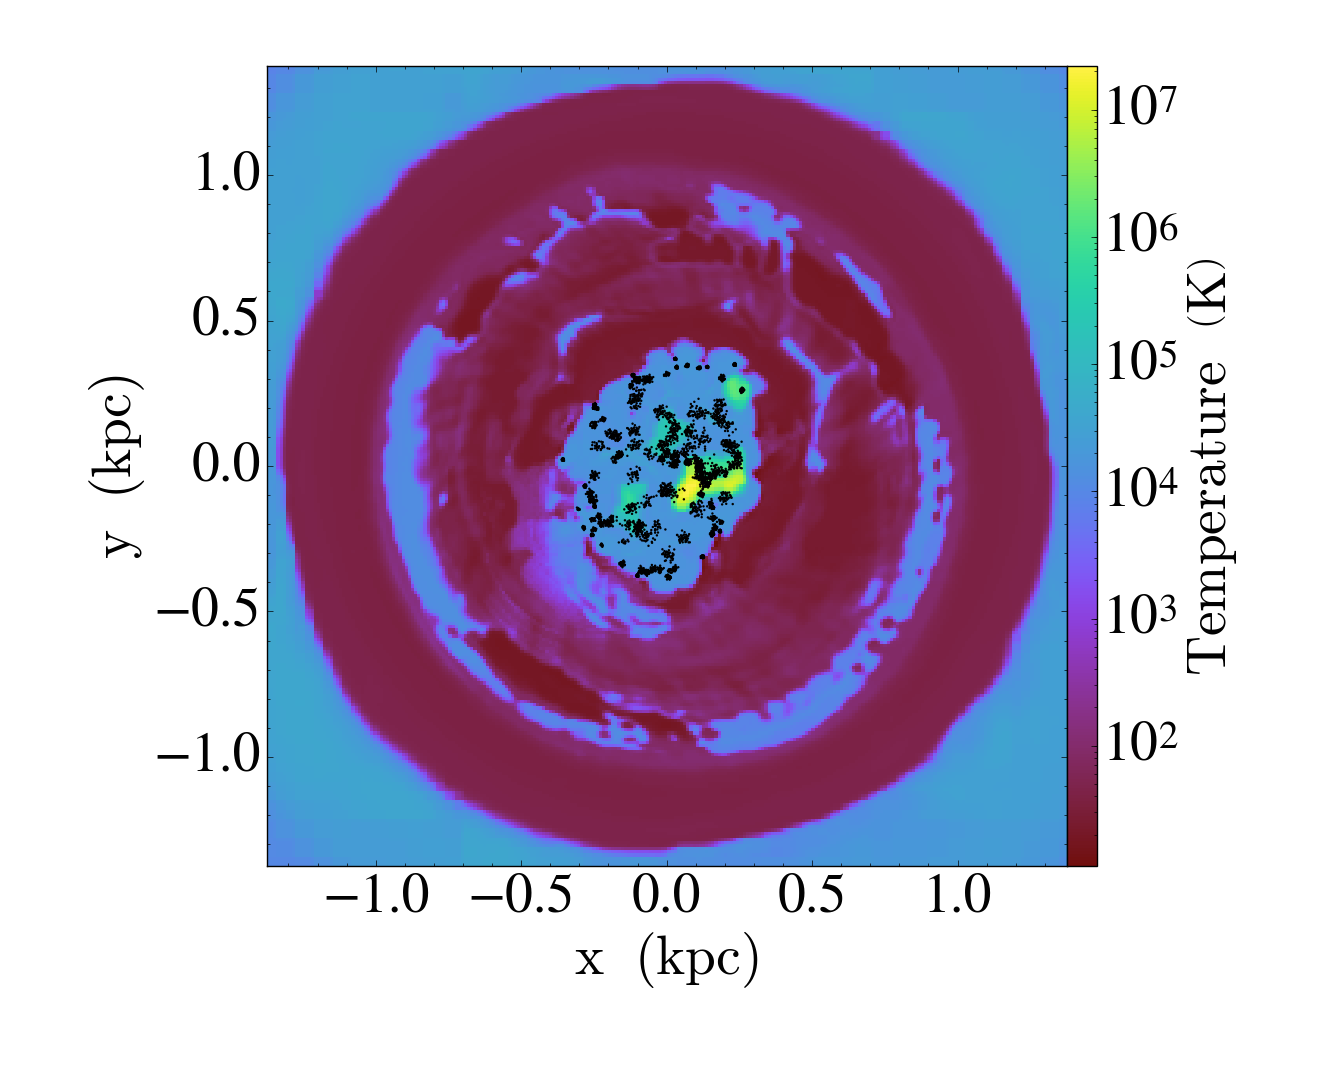
\includegraphics[width=0.4\linewidth]{temperature_slice}
\vspace{0.1cm}
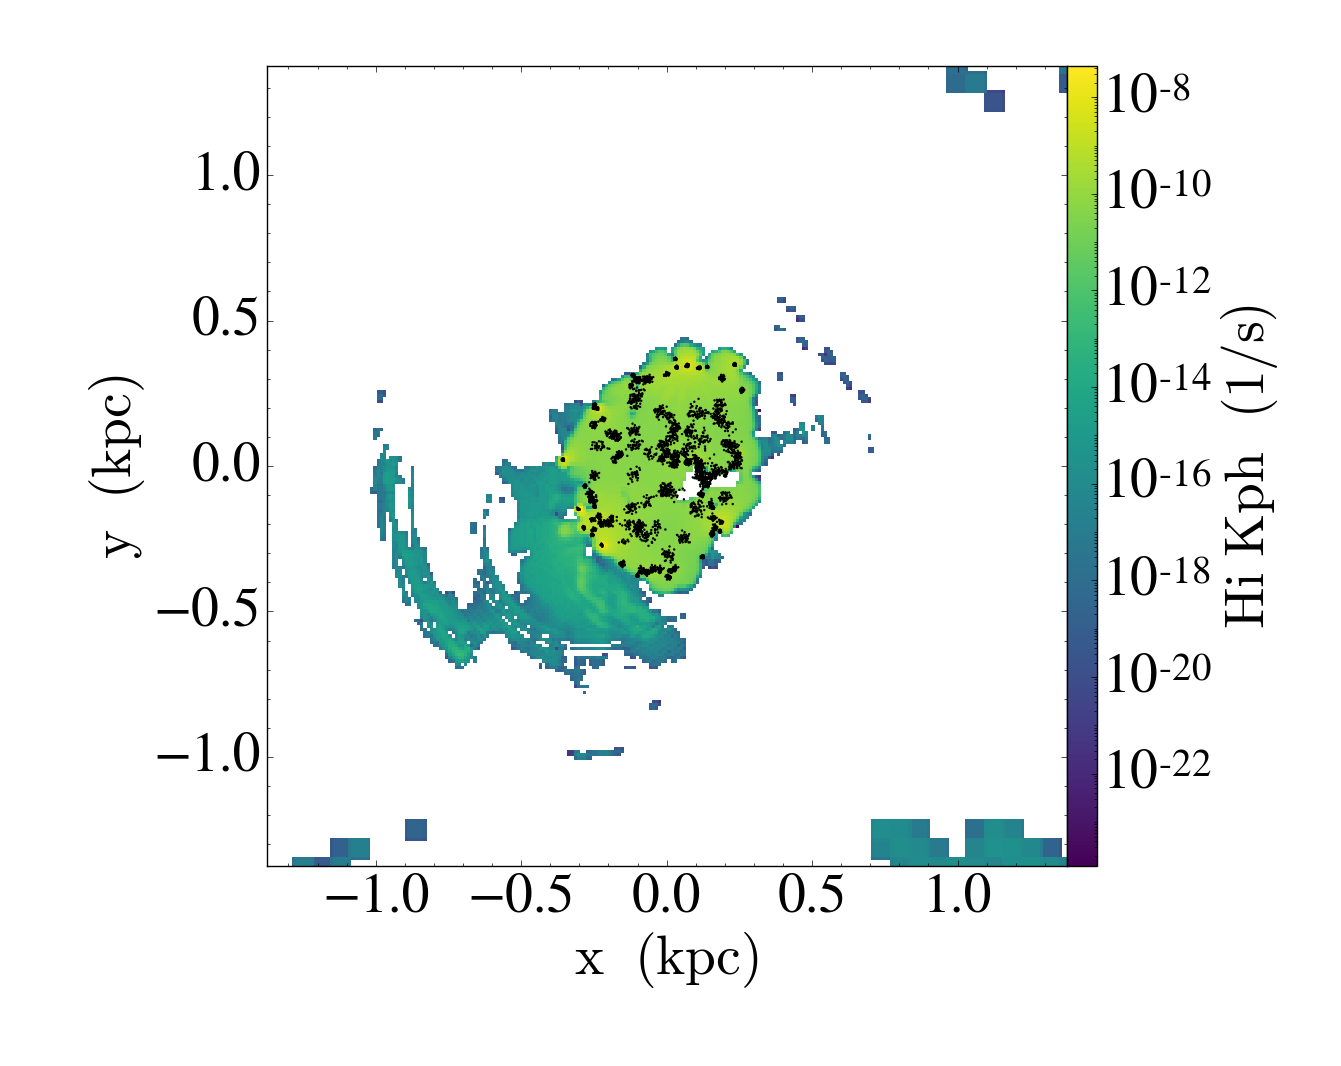
\includegraphics[width=0.4\linewidth]{hi_radiation_slice}
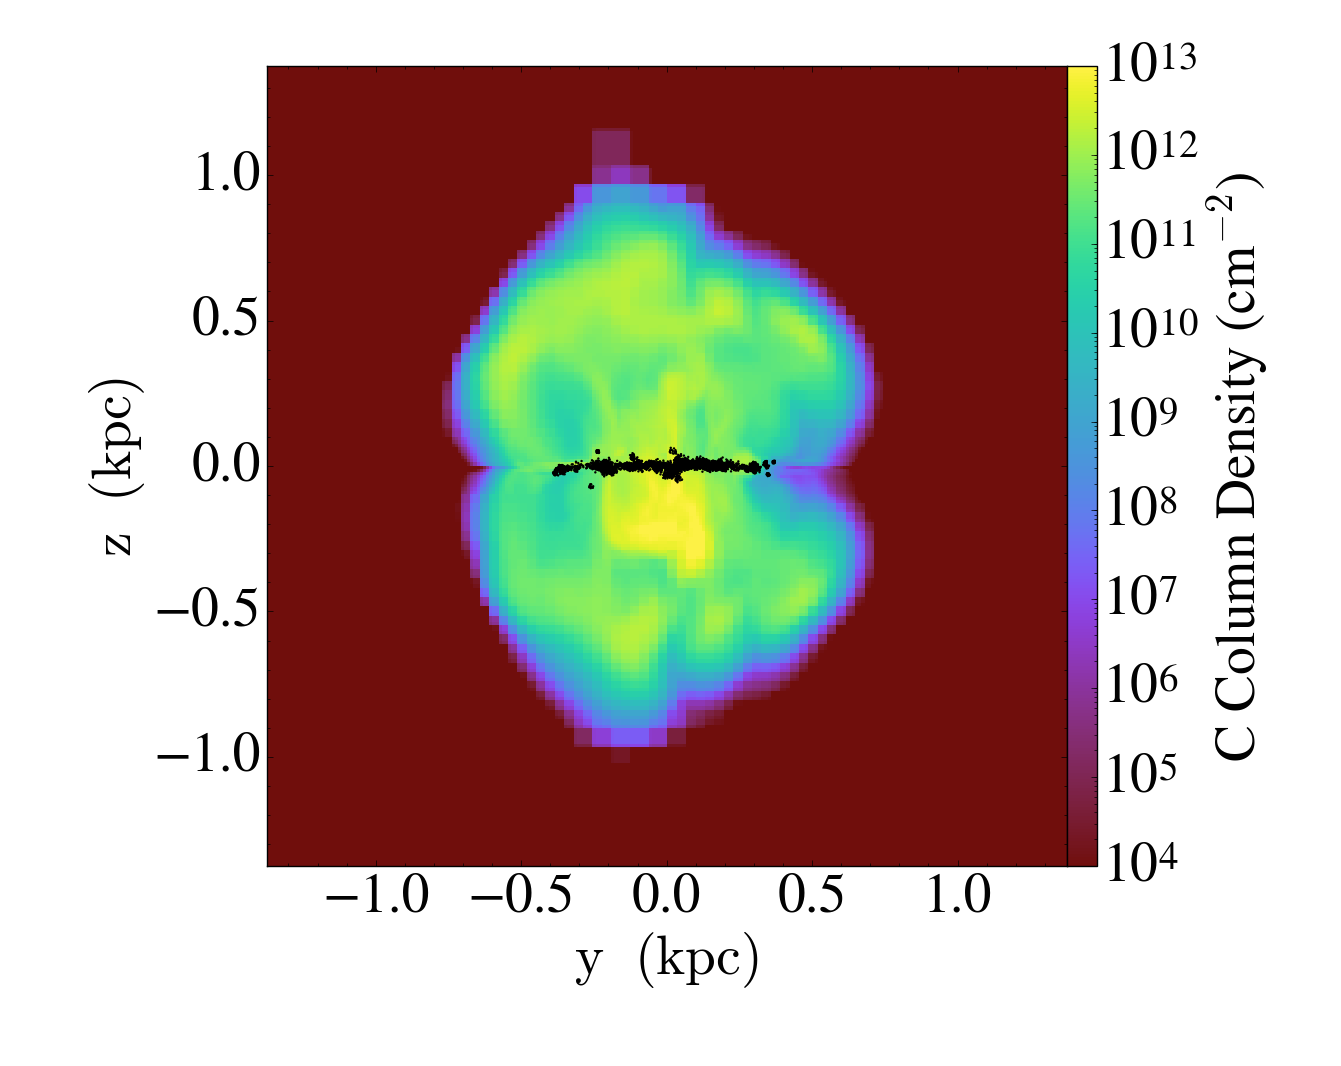
\includegraphics[width=0.4\linewidth]{c_projection}
\caption{\small Example images from a proof of concept test of our dwarf galaxy model at low resolution (8 pc). Shown here are face-on slices of number density (top left), temperature (top right), and H~{\sc i} ionizing radiation (bottom left), along with an edge-on projection of total carbon column density, illustrating yields ejected in metal enriched winds. This test was run with supernovae, stellar winds, radiative transfer, and photoelectric heating. Each black dot in the images is a star particle, which are often too clustered to distinguish between individual particles in these zoomed-out images. These images show the simulation $\sim$60 Myr after star formation, at which point there are 4,324 star particles with total mass $1.2\times10^4$ M$_{\odot}$. Of these, 173 are ionizing sources.}
\label{fig:dwarf galaxy}
\end{figure}

\section{Computational Resources}
***********************
We request a total of 9.68 million SU's and 12.3/2.6 TB of short/long term storage space, as explained below for each of our projects. Analysis for each project will be conducted on local computing resources utilizing the open source analysis toolkit \texttt{yt} \citep{yt}, and is therefore not considered in the total SU expense.

\subsection{Cluster Formation}

%\subsubsection{Scaling of the Code}

%The computational cost of our simulations is largely dominated by Flash, with our initial testing showing 10\% or less of the total simulation time spent outside of Flash. Specifically we expect our runs to be dominated by the ray tracing algorithm Fervent, which scales with the number of high mass stars (radiation sources) formed in the simulation. Fervent follows the original implementation by Wise and Abel \citep{wise_enzo+moray:_2011} by using asynchronous MPI calls where possible however. Our initial weak scaling of the code shows we are still getting speedup in Flash at 512 processors, and we expect to still scale well up to around 1K processors (Fig. \ref{fig:weakscale}).

%\subsubsection{Proposed Runs}

The cost of a single zone MHD update in Flash is about 150~$\mu$s. When radiation is added, this cost doubles \citep{WiseAbel2011}. Using the zoom algorithm, zooming in on the Bullhead cloud (mass $8 \times 10^3$~{\msun}) from kiloparsec scales down to $\sim50$~pc leaves us with about 2000 grids in the zoomed region. Further refinement levels each double the number of blocks from the previous level, since the volume filling factor is about 1/8th. It takes 12 levels of refinement to go to scales on the order of 100 AU. With $16^3$ cells per grid this gives about 8.3e7 cells total. The highest temperature on the grid generally will be from the winds, on the order of $10^6$~K. This gives a timestep of about 10~yr, and for a simulation run for 10~Myr requires $10^6$ steps. This leads to an estimate of total number of CPU hours of $11.5 \times 10^6$. Conducting this same estimate without winds means the highest temperature on the grid is generally due to the radiation at $10^4$ K (this anticipates that supernova are brief and infrequent events in our simulation). This leads to a total of $6.98 \times 10^5$ hrs for a single run. We therefore propose to do two runs for comparison, one with winds and one without.

% Saving the stuff below in case we want to request runs with carved out winds, etc.

%The cost of a single zone MHD update in Flash is about \SI{150}{\micro s}. When radiation is added, this cost doubles \citep{wise_enzo+moray:_2011}. Using the zoom algorithm, zooming in on the Bullhead cloud (mass \SI{8e3}{\msun})from \si{kpc} scales down to $\sim \SI{50}{pc}$ leaves us with about 2000 grids in the zoomed region. Further refinement levels each double the number of blocks from the previous level, since the volume filling factor is about 1/8th. It takes 12 levels of refinement to go to scales on the order of 100 \si{AU}. With $16^3$ cells per grid this gives about \num{8.3e7} cells total. The highest temperature on the grid generally will be from the winds, on the order of \SI{e4}{K}. This gives a timestep of about \SI{100}{yr}, and for a simulation run for \SI{10}{Myr} requires \num{e5} steps. This leads to an estimate of total number of CPU hours at \SI{6.98e5}{hrs}.

%If we make the rough approximation that a single cloud which is an order of magnitude more massive has double the radius (\SI{100}{pc} zoom in) and therefore about $2^3$ times as many initial grids, the same calculations lead us to estimate the number of CPU hours as \SI{1.4e6}{hrs}. With \num{1e4} processors, this run would take about 6 days on a large machine such as Stampede. For a cloud complex consisting of three clouds each of which is about \SI{2e5}{\msun} and contained inside a \SI{100}{pc} region, we can just assume the initial and zoomed number of grids is tripled, tripling the run time.

%\begin{widetext}

%\begin{tabular}{|c|c|c|c|}
\begin{table}
\centering
%\footnotesize
\begin{tabular}{|c|c|c|}
\hline 
Run \# & %Cloud & 
             Description & SU's ($\times 10^6$) \\
\hline 
1 & %$8 \times 10^3$~{\msun} & Bullhead cloud collapse - 
       All feedback & 11.5 \\
\hline 
2 & %$8 \times 10^3$~{\msun} & Bullhead cloud collapse - 
     Radiation and SN only & 0.7 \\
\hline 
%3 & \SI{8e3}{\msun} & Bullhead cloud collapse - Winds only & 700 \\
%\hline 
%4 & \SI{8e3}{\msun} & Bullhead cloud collapse - Supernova only & 7 \\
%\hline 
%5 & \SI{e5}{\msun} & Large cloud collapse with all feedback & 1400 \\
%\hline 
%6 & \SI{e6}{\msun} & 3 cloud complex collapse with all feedback & 4200 \\
\hline
%\multicolumn{3}{|c|}{Total Request} & 12200 \\
\multicolumn{2}{|c|}{Total Request} & 12.2 \\

\hline
\end{tabular}
\caption{\small Runs for the Flash/AMUSE combined simulations. One run with all forms of feedback will be run, along with a comparison run with only radiation and supernova.}
\end{table}


%\end{widetext}

%\begin{figure}
%\centering
%\includegraphics[width=1.0\linewidth]{weak_scale}
%\caption{Weak scaling of Flash running under AMUSE with Fervent. We gain approximately 15\% effeciency at 512 processors and expect the curve to flatten out around 10K processors.}
%\label{fig:weak}
%\end{figure}


\subsection{Feedback and Chemodynamics in Galaxies}

Our primary objective is to test the role various feedback processes play in the structural, dynamical, and chemical evolution of low mass dwarf galaxies. These simulations are tied to observable properties of nearby ultrafaint dwarf galaxies through star formation history, distribution and retention of chemical ejecta, and the spatial distribution and abundances of the individual stars. This is a pivotal test of whether or not widely used, approximate feedback methods are consistent with more physical descriptions of feedback, and more sensitive observational probes. The computational cost of these methods, and our requirement for high enough resolution to at least minimally resolve the feedback injection scales are the dominant grounds for the large number of SU's we require. From our test runs, a maximum resolution of 1.5 pc offers the best balance between resolving the feedback physics and available resources. These simulations will be vital for the understanding of feedback physics, and dwarf galaxy chemical and dynamical evolution, and can be used in future work to help implement physically motivated feedback methods in larger scale simulations. We outline the parameters and cost for each of our individual runs in Table~\ref{table:SU}, and discuss them in more detail below.

\begin{table}

 \centering
 \footnotesize

 \begin{tabular}{| R | R | R | R | R | r | r | r | R |}
 \hline
 \multicolumn{1}{|m{1.5cm}|}{Model Number} & \multicolumn{1}{m{1.2cm}|}{SN and Winds} & \multicolumn{1}{m{1.75cm}|}{Ionizing Radiation} & \multicolumn{1}{m{0.5cm}|}{Cosmic Rays} & \multicolumn{1}{m{1.25cm}|}{PE Heating} & Resolution (pc) & 10$^{3}$ SU/Myr & Time (Gyr) & \multicolumn{1}{m{1.0cm}|}{Total SU (10$^{6}$)} \\
 \hline

  1 & Y  & N & N & N & 1.5 & 0.24 & 1.0 & 0.24 \\
  2 & Y* & N & N & N & 1.5 & 0.12 & 1.0 & 0.12 \\
  3 & Y  & Y & N & N & 1.5 & 2.4  & 1.0 & 2.4 \\
  4 & Y  & N & Y & N & 1.5 & 1.2  & 1.0 & 1.2 \\
  5 & Y  & N & N & Y & 1.5 & 0.24 & 1.0 & 0.24 \\
  6 & Y  & Y & N & Y & 1.5 & 1.2  & 1.0 & 1.2 \\
  7 & Y  & Y & Y & Y & 1.5 & 3.0  & 1.0 & 3.0 \\
  8 & Y  & Y & Y & Y & 0.75 & 12 & 0.1 & 1.2  \\
  9 & Y  & Y & Y & Y & 3.0 & 0.75 & 0.1 & 0.08  \\
  \hline
  Total & - & - & - & - & - & - & - & 9.68  \\
 \hline
 \end{tabular}

 \caption{\small List of our planned dwarf galaxy feedback simulations and the various processes included in each. Stellar winds and supernovae are consistent in each case, except in model 2, where we ignore stellar wind energy injection (see text). Each simulation has a maximum spatial resolution of 1.5 pc with the exception of models 8 and 9, which will be run for a shorter time at 0.75 and 3.0 pc resolution respectively.}
   \label{table:SU}
\end{table}

\begin{table}
 \centering
 \footnotesize
 \begin{tabular}{| R | R | R | R | R | R | R  | R }
 \hline
 \multicolumn{1}{|m{1.5cm}|}{Model Number} & \multicolumn{1}{m{1cm}|}{Number of Fields} & \multicolumn{1}{m{2.25 cm}|}{Number of Particle Fields} & \multicolumn{1}{m{2.0cm}|}{Memory Per Output (Gb)} & \multicolumn{1}{m{1.75 cm}|}{Short / Long Term Cadence (Myr)} & \multicolumn{1}{m{1.5cm}|}{Short Term Storage (TB)} & \multicolumn{1}{m{1.5cm}|}{Long Term Storage (TB)} \\
 \hline

  1 & 33 & 25 & 2.7 &  2.5 / 10 & 1.12 & 0.28  \\
  2 & 33 & 25 & 2.7 &  2.5 / 10 & 1.12 & 0.28  \\  
  3 & 40 & 25 & 3.2 &  2.5 / 10 & 1.35 & 0.34  \\
  4 & 34 & 25 & 2.7 &  2.5 / 10 & 1.15 & 0.29  \\
  5 & 35 & 25 & 2.8 &  2.5 / 10 & 1.18 & 0.30  \\
  6 & 42 & 25 & 3.4 &  2.5 / 10 & 1.42 & 0.35  \\
  7 & 43 & 25 & 3.5 &  2.5 / 10 & 1.45 & 0.36  \\
  8 & 43 & 25 & 33  &  0.5 / 5  & 3.48  & 0.35  \\  
  9 & 43 & 25 & 1.75 & 2.5 / 10  & 0.03 & 0.01 \\
  \hline
  TOTAL & - & - & - & - & 12.3 & 2.6 \\
 \hline
 \end{tabular}
 \caption{\small The estimated short and long term memory storage requirements for each of our dwarf galaxy simulations, and the total storage requested for this portion of our project. Each of the above grid and particle fields are stored as a 64 bit float. The above calculations are made assuming a typical grid cell count of $1.05\times 10^{7}$ and particle count of $\sim 10^{5}$. For our short, high resolution simulation (model 8) we expect on order of $\sim5\times 10^{7}$ grid cells, and $\sim2 \times 10^{6}$ in model 9. Our 1 Gyr runs (models 1 - 7) will have a total of 400 short term and 100 long term outputs, and our short resolution study runs will have 200 short term and 20 long term outputs.}
 \label{table:storage}
\end{table}

We trace a total of twelve metal abundances in each simulation, restricting ourselves to those most readily constrained by observations, while adequately sampling signatures of distinct nucleosynthetic processes \citep[see][and references therein]{Tolstoy2009}: C, N, O, Mg, Si, S, Mn, Fe, Ni, Y, Ba, and Eu. Stellar winds and supernovae are treated consistently in all models, with the exception of model 2. In model 2 we test the global importance of stellar wind feedback, leaving metal pollution by stellar winds on, but ignoring their energy injection into the ISM. Each subsequent simulation, models 3 through 6, varies the combination of feedback physics included, which we separate into ionizing radiation (radiative transfer), CRs, and photoelectric heating. Model 7 combines all of these mechanisms in a single simulation. Finally, we perform a resolution test at higher resolution (model 8) and lower resolution (model 9) to better understand the limitations even 1.5 pc resolution places on these processes. As indicated in Table~\ref{table:SU}, the additional estimated computational expense of a 0.75 parsec resolution simulation restricts us to a reduced simulation time of 100 Myr. For this reason, we will use one of the model 7 outputs at $\sim$500 Myr as the initial conditions of model 8, to ensure all feedback mechanisms are active for a more faithful resolution study. For consistency, we will simulate the 3.0 pc low resolution model (model 9) over the same period of time, but for a small fraction of the cost.

The SU / Myr cost of each simulation is controlled by the total number of grid cells, size of each time step, and whether or not radiative transfer is included. We estimate that the high velocity stellar winds (10$^{2-3}$ km s$^{-1}$) and hot gas from supernovae and shocks (10$^{6-7}$ K) will restrict the the maximum refinement level to time steps on order of a few to several hundred years. Based upon our initial tests at 1.0 and 2.0 pc resolution, we estimate the 1.5 pc simulations will contain approximately 1.05$\times$10$^{7}$ cells, a majority of which would be on the highest refinement level. Our scaling tests show \texttt{Enzo} operates at $\sim 2\times10^{4}$ cell updates per second per processor (without radiative transfer and CR's). We expect to run on 128 processors for a majority of the simulation time, giving a total cell update rate of roughly 2.56$\times 10^{6}$ cells per second across all processors. For a time step of 600 years, this equates to about 1.9 wall hours per Myr, or for 128 processors, about 243 SU / Myr, and roughly 0.24 million hours per Gyr. These numbers are reflected in model 1 in Table~\ref{table:SU}. The additional cost of PE heating is insignificant, and may actually decrease total simulation time, as the additional heating may prevent some star formation. We estimate removing energy injection from stellar winds will increase the average time step by about a factor of two over the course of a simulation. As discussed previously and in more detail in our supporting document, we expect radiative transfer to be about an order of magnitude more expensive. Tracking CR energy density adds little additional computational cost per timestep, but will decrease the typical timestep by a factor of about 5, thus increasing the total cost by about 5. These estimated values were all derived using both prior experience working with these methods from collaborators, as well as our low resolution 8.0 pc test simulation.

We plan to run each simulation for 1 Gyr, saving data dumps every 2.5 Myr. We estimate that this cadence is necessary to provide access to 2--10 restart dumps within a single job submission (depending on the included physics). Rapid analysis of this high cadence will allow us to understand the short timescale variance of dwarf galaxy chemodynamics; these will also be used to make high time resolution movies of our simulation set. Each output contains all of the information about the simulation at a single time. The memory required for each dump varies depending on the physics used, as follows. Each simulation dump will contain 11 fields associated with the hydrodynamics and 22 fields associated with the primordial chemistry and metal abundance tracers, for a base total of 33. Radiative transfer (ionizing radiation) simulations will contain an additional 7, while photoelectric heating and Lyman Werner radiation add an additional 2. CRs only add a single additional field, for a total of 43 fields per cell in our full physics simulations. In addition, each particle keeps track of 25 properties, 15 of which are abundances (metallicity, H, He, and metal tracers), while the rest include position (3), velocity (3), current mass, birth mass, lifetime, and formation time. Taking into account these values, our output cadence, the expected grid size of around $10^7$ cells, and the expected $\sim$10$^{5}$ star particles, we present our estimated memory storage requirements in Table~\ref{table:storage}. \texttt{Enzo} operates in double precision; to ensure accuracy during restarts and to prevent loss of precision, each of our output dumps will also be in double precision.

\section{Project team qualifications}

\textbf{PI: Mordecai-Mark Mac Low}  is a tenured curator in the Department of Astrophysics at the American
Museum of Natural History in New York, as well as holding an adjunct professorship in the Department of 
Astronomy at Columbia U.  He was awarded a Humboldt Prize to visit the University of Heidelberg in 2015-2016.
He worked with and participated in the
development of the astrophysical MHD code Zeus starting in 1986, including
developing a module to include ambipolar diffusion
% (Mac Low et al. 1995; Mac Low \& Smith 1997), 
\citep{MacLow1995,MacLowSmith1997} and writing the first version of MHD
for Zeus-MP 
%(Hayes et al.\ 2006)
\citep{Hayes2006}.  He has also published work using GADGET 
%(Li, Mac Low \& Klessen 2005ab, 2006).  
\citep{Li2005,Li2005a,Li2006},
the Pencil code 
%(Oishi, Mac Low, \& Menou 2007; Johansen et al.\ 2007; Johansen, Youdin, \& Mac Low 2009; Yang, Mac Low, \& Menou 2009; Oishi \& Mac Low 2009,McNally et al. 2014), 
\citep{Oishi2007,Johansen2007,Johansen2009,Yang2009,OishiMacLow2009,McNally2014}, and
Flash 
%(Joung \& Mac Low 2006; Joung et al.\ 2009;Peters et al.\ 2010abc, 2011, 2012, Hill et al. 2012),
\citep{Joung2006,Joung2009,Peters2010,Peters2010a,Peters2010b,Peters2011,Peters2012,Hill2012,Gatto2015,Girichidis2016SImulatingOutflows,Ibanez-Mejia2016}, and Enzo \citep{Simpson2013}.
In
total, he has published over 130 refereed papers. He is co-supervisor of the dissertation work of both co-PIs, and
will supervise the work proposed here, ensuring completion and publication.

\textbf{co-PI: Andrew Emerick} is a PhD student at Columbia University advised by both PI Mac Low and collaborator Greg Bryan. Emerick is the developer of the new star formation, feedback, and stellar yield models used in the isolated dwarf galaxy simulations and drafted these sections of the proposal. This work is central focus of his thesis research. Previously he has published research working with \texttt{ENZO}, making synthetic absorption observations of gas in simulated galaxy clusters \citep{Emerick2015}, and \texttt{FLASH}, studying gas stripping and feedback in low mass dwarf galaxy satellites of the Milky Way \citep{Emerick2016}.

\textbf{co-PI: Joshua Wall} is a PhD student at Drexel University advised by both PI Mac Low and collaborator Stephen McMillan. Wall has developed the interface for Flash into AMUSE, the gravity bridge for Flash and the N-body code, the supernova and wind algorithms in Flash, and modified FERVENT to couple to sink particles and include radiation pressure. He has experience in programming and building MPI parallel computing applications on many different high performance clusters. Further he has worked on two previous computing resource grants, one from NASA's HEC program and a second at SurfSARA in the Netherlands. %Collaborator Wall is in his fourth year of his PhD and is anticipated to graduate in 2017.

\textbf{Collaborator: Greg Bryan} is a professor at Columbia University and a Research Scientist at the Simons Center for Computational Astrophysics at the Flatiron Institute. Bryan was the original author of the \texttt{Enzo} simulation code, and continues to play an active role in its development. % {\bf additional text / rewording TBD}.

\textbf{Collaborator: Stephen McMillan} is a professor and acting chair of the Department of Physics at Drexel University.  He was the original author of the ph4 N-body code, and has been a central member of the collaboration developing the AMUSE framework from its inception.

\section{Management}

\subsection{Summary}

Code development, production, and analysis of simulations of star cluster formation Flash + AMUSE will be led by co-PI Wall. This project is in collaboration with broader code development efforts at the Flash Center of the U. of Chicago, R. Klessen's group at the Institute for Theoretical Astrophysics of the University of Heidelberg, and S. Portegies-Zwart's group at Leiden University.  

Code development, production, and analysis of simulations of star formation, feedback, and chemodynamics of isolation galaxies in \texttt{Enzo} will be led by co-PI Emerick. These simulations will be supervised by PI Mac Low and collaborator Greg Bryan. This project relies on collaboration and advice from many additional researchers, including Brian O'Shea (Michigan State), Benoit C{\^o}t{\'e} (Michigan State), Mary Putman (Columbia), Kathryn Johnston (Columbia), Britton Smith (Edinburgh), John Wise (Georgia Tech), and Simon Glover (ITA-Heidelberg).

\subsection{Local Computing Environment}

The PI's group has an analysis workstation containing  2 AMD 6344 Abu Dhabi processors with 12 cores each, 256 GB of memory, 16 TB of data space, about 40 GB of home directory space, and an Nvidia GeForce GT 610 graphics card. It is running Ubuntu, and has all standard libraries installed.  The PI and his group also have partial access to two small clusters at the Museum. These include a 128 core (32 nodes each with two dual core processors) Xeon cluster connected with Infiniband, and a 40-processor Sunfire Ultrasparc III 900 Mhz cluster. These aged machines are shared with other users at the Museum including biologists doing large phylogenetic computations, and other astrophysicists.

Through the Department of Astronomy at Columbia University, co-PI Emerick has partial access to Yeti, a 2762 core (167 nodes with dual, 1.8 Ghz, 8 core processors) HPC cluster. A subset, 64, of these nodes are connected via Infiniband. Resources on this cluster are shared between several departments at Columbia on a department-by-department basis. The ease of access coupled with fairly short to no queue wait times makes this an ideal resource for code development, testing, and some analysis work. However, resource availability and ``fair-use'' principles make using Yeti for production level simulations prohibitive. Some short term storage is available on this cluster, but is severely limited; a total of 5 TB is shared between $\sim$ 50 users.

Through the Physics Department at Drexel University, co-PI Wall as has partial access to a 24 node Beowulf cluster with 288 Westmere cores and 128 Nvidia GPUs. This cluster is shared among the seven graduate students of the computational astrophysics group at Drexel. All members of the group utilize the cluster for large parallel codes in hydrodynamics or N-body studies. Generally co-PI Wall has access to a few nodes (24-48 cores) on this machine for development of code. Drexel University also has a 2496 core mixed processor AMD / Intel cluster that is utilized university wide by all departments. Biology and a few other departments permanently reserve the use of a number of the nodes on this machine, and all other users are restricted to 512 cores for 48 hours of runtime at a time. The machine is heavily oversubscribed throughout the university, with queue times on the order of weeks. This prohibits usage for production level runs.

\subsection{Other Supercomputing Support}

Wall (project leader) and Mac Low are coinvestigators with S. Portegies-Zwart (PI), R. Klessen,  S. McMillan, and J. Ib\'a\~nez-Mej\'{\i}a on a 4M SBU allocation on the Dutch NWO supercomputer at SurfSARA.  We plan to use this allocation to do a model neglecting stellar winds of a cloud an order of magnitude more massive than the one proposed here.

Wall (project leader) and Mac Low are also coinvestigators with S. McMillan (PI), and J. Ib\'a\~nez-Mej\'{\i}a on a NASA Science Mission Directorate HEC proposal for 5M SBU (409,000 Pleiades SBUs) to study the effects of gas ejection from natal clusters on the long term evolution of the cluster. Where we focus on here on early evolution and star formation efficiency (up to about 10 Myr), on Pleiades we intend to run lower resolution but much longer post gas ejection.
 
Emerick has completed an XSEDE startup grant, which supported some of his work on ram pressure stripping as noted in the progress report.

\clearpage
\bibliographystyle{apj}
\bibliography{msAllbib}


\end{document}
